\chapter{State of the art}
\label{ch:state-of-the-art}
Time series are a type of data that indicate how things change over time. They are different from other types because time is a fundamental dimension on them, being data order as important as the data per se. That's why analyzing and forecasting time series is more challenging and extra considerations should be taken into account. \cite{lazzeri2020machine}

\section{Time series components}
The three components that conform them are:
\begin{itemize}
    \item Trend component ($T_t$): Defined as the long term movement in a time series. It can be constant, increasing or decreasing in time.
    \item Seasonal component ($S_t$): Periodic fluctuations in the series that normally happen in a period of less than a year. Weather seasons or social conventions are examples of what produces this seasonality.
    \item Cyclic component ($C_t$): Recurrent fluctuations that appear in the series but don't have a fixed length. An example of this is a business cycle, whose duration is not known a priori.
    \item Remainder component ($R_t$): Unpredictable variations that can not be explained by the other three.
\end{itemize}

They can be combined in an additive way ($y_t = S_t + C_t + T_t + R_t$), a multiplicative one ($y_t = S_t \times C_t \times T_t \times R_t$) or a combination of both ($y_t = S_t \times C_t + T_t + R_t$, $y_t = S_t + C_t + T_t \times R_t$\ldots). The additive decomposition is more adequate when the degree of variation in the components doesn't seem to change with the level of the time series. Otherwise, is more recommended to apply a multiplicative one.  \cite{hyndman2018forecasting,lazzeri2020machine}

\subsubsection{Stationarity}
A very important concept in time series is stationarity.
A stationary time series is one whose properties does not change with time, with the moment in which the series is observed. If some trend or seasonality is present, it doesn't hold.

Usually, a stationary time series will have no predictable patterns in the long term. Nevertheless, a cyclic behaviour with no trend nor seasonality is stationary.

One way of detecting stationarity is by generating ACF plots. These are also useful to detect seasonality in the series. \cite{hyndman2018forecasting}


\section{Forecasting}
In \cite{hyndman2018forecasting}, the author explains that "forecasting is about predicting the future as accurately as possible, given all the information available, including historical data and knowledge of any future events that might impact the forecasts".

When forecasting, it's needed to know how many steps in the future want to be predicted. This is called the forecasting horizon, and can be composed of just one or multiple steps.

Other important aspect to consider is the forecasting method to use. Which one to choose will depend on the characteristics of the time series, using simpler or more advanced methods.


\subsection{Simple methods}
In some situations they can be effective. Some of these methods are: \cite{hyndman2018forecasting}
\begin{itemize}
    \item \textbf{Average method:} Forecast with the mean of the historical data. A very popular variation of this technique is the Moving Average (MA) method, in which the mean is computed not over the complete historical series but over the K more recent points.
    \item \textbf{Naïve method:} Forecast with the last observation of the historical data.
    \item \textbf{Drift method:} A modification of the previous technique where forecasts increase or decrease over time.
\end{itemize}

\subsection{Classical methods}
These methods were developed some decades ago and are based on statistics. They have been the de facto standard to forecast time series until the creation of more advanced methods. Some of them are: \cite{lazzeri2020machine, hyndman2018forecasting}
\begin{itemize}
    \item \textbf{Exponential smoothing (ETS):} Uses the MA method, assigning higher weights to more recent values and lower weights to those which are more distant in time. Combines Error, Trend and Seasonality components to model the series.
    \item \textbf{Auto Regressive Integrated Moving Average (ARIMA):} Combines an autoregressive model, in which a linear model is trained using as predictors the lagged values of the variable, with a moving average and integration. In the moving average, instead of forecasting using lags of the actual variable, past forecasting errors are used as predictors. The integration step is in charge of making the time series stationary.
\end{itemize}

\subsection{More advanced methods}
The development in Machine Learning (ML) also arrived to time series, being models such as Random Forest, k-Nearest Neighbours or LSTM used to forecast the future \cite{lazzeri2020machine}.
In classical time series models as ARIMA data can be directly introduced in the model without restructuring it: but when using ML-based architectures, data has to be reshaped so the models can recover autocorrelation.

See Figure \ref{fig:ml-arrangement}.
On it, the response (price) and predictors (as could be demand or generation) are included together with some response lags, acting as predictors too.
This data structure is what is used as input for the ML models, not the raw data itself.

\begin{figure}[H]
\centering
    \caption{Tabular form in which data is disposed for ML models. On it, n is the number of observations in the time series and k is the number of lags in use.}
    \label{fig:ml-arrangement}
    \fbox{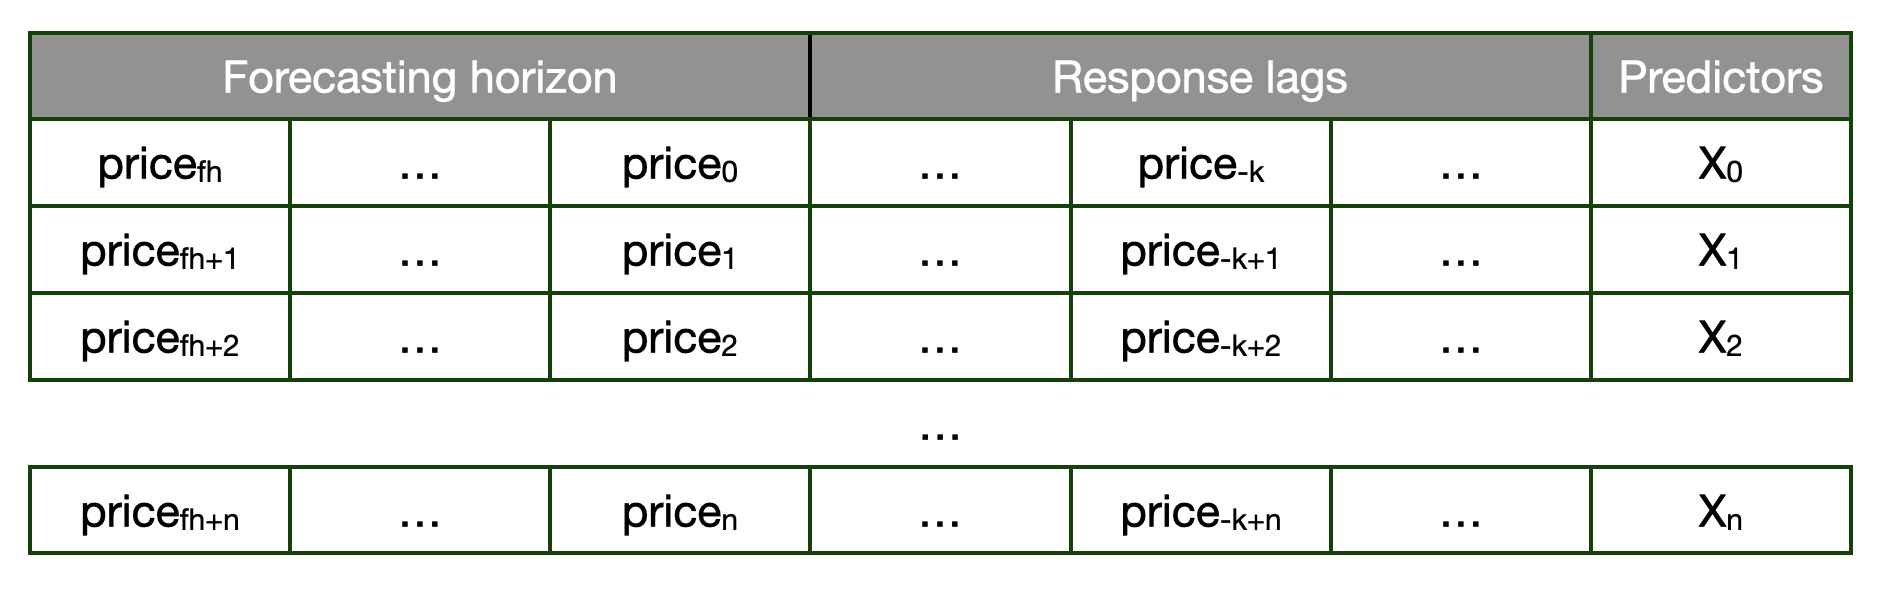
\includegraphics[scale=0.4]{images/methodology/ml_arrangement}}
\end{figure}

\noindent Some ML models that could be used to forecast are the following: \cite{berzal2018redes}
\begin{itemize}
    \item \textbf{k-Nearest Neighbors (kNN):} Distance-based algorithm which computes the label of a new observation as the mean of the labels of the k closer training observations. It is known as a lazy learner, in the sense that it doesn't build a proper model, but it directly uses the training data to classify new observations.
    \item \textbf{Support Vector Machines (SVM):} Also known as large margin classifiers, SVMs are algorithms that try to model a function that deviates from the training responses no more than a distance epsilon, while the curve remains the flattest possible.
    \item \textbf{Random Forests (RF):} Ensemble method in which several decision trees are trained over a different subset of the training set, using a random set of predictors. The final prediction is built as the average of the individual decision trees results.
    \item \textbf{Gradient Boosted Trees (GBT):} Ensemble method based on boosting. The goal is to iteratively add new decision trees to the ensemble, improving it. Each training instance has assigned a different weight: those which are more difficult to classify will have a higher weight and the trees added in following iteration will focus more on them.
\end{itemize}

\subsection{Error metrics}
To asses the quality of a forecast it is necessary to define an error metric. This is an important step, as different metrics will penalize different aspects of the forecast. In the context of time series, these are some widely used: \cite{hyndman2006another,ts-metrics-formulas}
\begin{itemize}
    \item \textbf{Mean Absolute Error (MAE):}
    \begin{equation}
        \label{eq:mae}
        \text{MAE}(y, \hat{y}) = \frac{ \sum_{i=0}^{N - 1} |y_i - \hat{y}_i| }{N}
    \end{equation}
    This metric, as it names indicates, is computed from the absolute difference between the observed and forecasted value. It is a scale-dependent measure, so it can't be used to compare series with different units. It ranges from 0 to $+\infty$, being 0 the smallest error.
    \item \textbf{Mean Absolute Percentage Error (MAPE):}
    \begin{equation}
        \label{eq:mape}
        \text{MAPE}(y, \hat{y}) = \frac{100\%}{N} \sum_{i=0}^{N - 1} \frac{|y_i - \hat{y}_i|}{|y_i|}.
    \end{equation}
    Similar to the previous metric but scale-independent, this is why it can be a good option to compare series with different units. Nevertheless, it comes with two major drawbacks. When the true value $y_i$ is close to 0, this metric becomes undefined. Apart, it puts a heavier penalty on positive than on negative errors. It ranges from 0 to $+\infty$.
    \item \textbf{Mean Absolute Scaled Error (MASE):}
    \begin{equation}
        \label{eq:mase}
        \text{MASE}(y, \hat{y}) = \frac{1}{N}\sum_{k=1}^{N}\frac{|p_k-\hat{p}_k|}{\frac{1}{n-1}\sum_{i=2}^{n} |p^\mathrm{in}_i - p^\mathrm{in}_{i-1} |},
    \end{equation}
    Scale-independent measure. It is only undefined in the case of all historical observations being equal. Again, it ranges from 0 to $+\infty$.

\end{itemize}

\noindent In Chapter \ref{ch:methodology}, we will discuss which models are more adequate for our problem and which is the most suitable metric between those presented here. In addition, other eminently practical questions on the design of the methodology will be addressed.

\section{Model explainability}
%When forecasting (and predicting in general) it is important to build a model that adequately captures the underlying patterns of data. This will lead to accurate and strong predictions.
%
%But in many cases it is also important to understand how data is affecting the model. Which variables are more important in the prediction? How and why? This is an issue that model interpretability attempts to solve. A way of achieving this is using SHAP values.

The goal of this project is not just to forecast electricity prices, but also to understand which variables are influencing them. The challenge with many models is that they act as a black box, so understanding why some variables are more or less important in the final prediction is not straightforward.

This is what SHapley Additive exPlanations (SHAP) \cite{lundberg2017unified} values try to overcome. On them, features are treated as players that participate in a game. The game consists in replicating the output of the model, checking what is the contribution of each player to the final result. This game is repeated for each data observation individually \cite{shap-simplified}. This method is fascinating as no internal knowledge of the model is required, we just need to know the model inputs and output.

Obtaining the SHAP values will enable us to explain how the predictors influence the forecast.


%sktime \cite{DBLP:journals/corr/abs-1909-07872}
%pmdarima \cite{pmdarima}
%scikit-learn \cite{scikit-learn}
%SHAP package \cite{shap-package}
